% Dit werk is gelicenseerd onder de licentie Creative Commons Naamsvermelding-GelijkDelen 4.0 Internationaal. Ga naar http://creativecommons.org/licenses/by-sa/4.0/ om een kopie van de licentie te kunnen lezen.
\chapter{Tabellen en grafieken}
\label{sec:Tabellen en grafieken}

\makeatletter
\setlength{\@fptop}{0pt}
\makeatother
\captionsetup{justification=justified,singlelinecheck=false}
\raggedbottom

\begin{minipage}{\textwidth}
	\captionof{table}{Verliescoëfficiënt bij stroming door een cirkelvormige bocht van 90\deg \\ $h_\mathrm{L} = K \frac{v^2}{2g}$}
	\begin{tabular}[t]{p{12cm} p{5cm}}
		\begin{tabular}{l c c c c c}
			$r/D$        & 1    & 2    & 4    & 6    & 10   \\
			\hline
			$K$ glad & 0.21 & 0.14 & 0.11 & 0.09 & 0.11 \\
			$K$ ruw  & 0.51 & 0.30 & 0.23 & 0.18 & 0.20
		\end{tabular}
		&
		\smash{\raisebox{-0.5\height}{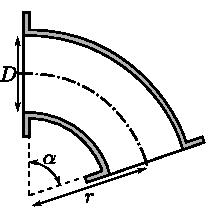
\includegraphics{fig/appendix/Bocht}}}
	\end{tabular}
\end{minipage}

\begin{minipage}{\textwidth}
	\captionof{table}{Correctiefactor voor cirkelvormige bochten met andere hoeken \\ $h_\mathrm{L} = f K_{90\deg} \frac{v^2}{2g}$}
	\begin{tabular}[t]{p{12cm} p{5cm}}
		\begin{tabular}{l c c c c c c}
			$\alpha$ & 30\deg & 60\deg & 90\deg & 120\deg & 150\deg & 180\deg   \\ 
			\hline
			$f$    & 0.4    & 0.7    & 1      & 1.25    & 1.5     & 1.7
		\end{tabular}
		&
	\end{tabular}
\end{minipage}


\begin{minipage}{\textwidth}
	\captionof{table}{Verliescoëfficiënt voor een plotse verwijding \\ $h_\mathrm{L} = K \frac{v_1^2}{2g}$}
	\begin{tabular}[t]{p{12cm} p{5cm}}
		\begin{tabular}{l c c c c c c c c c}
			$D_2/D_1$ & 1.0 & 1.2 & 1.4 & 1.6 & 1.8 & 2.0 & 3.0 & 5.0 & $\infty$ \\ 
			\hline
			$K$    & 0.00    & 0.09    & 0.24      & 0.37    & 0.48     & 0.56 & 0.79 & 0.92 & 1.00
		\end{tabular}
		&
		\vfill
		\smash{\raisebox{-0.5\height}{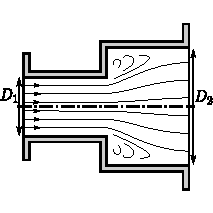
\includegraphics{fig/appendix/Verwijding}}}
	\end{tabular}
\end{minipage}
\vspace{1cm}

\begin{minipage}{\textwidth}
	\captionof{table}{Correctiefactor voor een geleidelijke verwijding \\ $h_\mathrm{L} = f K_{180\deg} \frac{v_1^2}{2g}$}
	\begin{tabular}[t]{p{12cm} p{5cm}}
		\begin{tabular}{l c c c c c c c c c c}
			$\alpha$ & 6\deg & 10\deg & 15\deg & 20\deg & 30\deg & 40\deg & 50\deg & 60\deg & 70\deg & 90\deg \\ 
			\hline
			$f$    & 0.14    & 0.20    & 0.30      & 0.40    & 0.70     & 0.90 & 1.00 & 1.10 & 1.10 & 1.00
		\end{tabular}
		&
		\vfill
		\smash{\raisebox{-0.5\height}{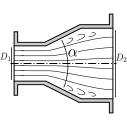
\includegraphics{fig/appendix/Gelijdelijke_verwijding}}}
	\end{tabular}
\end{minipage}
\vspace{1cm}

\begin{minipage}{\textwidth}
	\captionof{table}{Verliescoëfficiënt bij stroming door een plotse vernauwing \\ $h_\mathrm{L} = K \frac{v_2^2}{2g}$}
	\begin{tabular}[t]{p{12cm} p{5cm}}
		\begin{tabular}{l c c c c c c c c c}
			$D_1/D_2$ & 1 & 	1.2 & 	1.4 & 	1.6 & 	1.8 & 	2.0 & 	3.0 & 	5.0\\
			\hline
			$K$  & 0.00 & 	0.15 & 	0.24 & 	0.30 & 	0.35 & 	0.38 & 	0.44 & 	0.48
		\end{tabular}
		&
		\vfill
		\smash{\raisebox{-0.5\height}{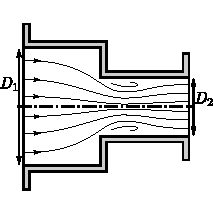
\includegraphics{fig/appendix/Vernauwing}}}
	\end{tabular}
\end{minipage}
\vspace{1cm}

\begin{minipage}{\textwidth}
	\captionof{table}{Correctiefactor voor een geleidelijke vernauwing \\ $h_\mathrm{L} = f K_{180\deg} \frac{v_2^2}{2g}$}
	\begin{tabular}[t]{p{12cm} p{5cm}}
		\begin{tabular}{l c c c c c c}
			$\alpha$ & 45\deg & 60\deg & 90\deg & 120\deg & 150\deg & 180\deg \\ 
			\hline
			$f$    & 0.62	& 0.71 & 	0.84 &	0.93 &	0.98 &	1.00 \\
		\end{tabular}
		&
		\vfill
		\smash{\raisebox{-0.5\height}{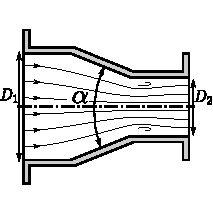
\includegraphics{fig/appendix/Gelijdelijke_vernauwing}}}
	\end{tabular}
\end{minipage}
\vspace{1cm}

\begin{minipage}{\textwidth}
	\captionof{table}{Verliescoëfficiënt voor een orifice \\ $h_\mathrm{L} = K \frac{v^2}{2g}$}
	\begin{tabular}[t]{p{12cm} p{5cm}}
		\begin{tabular}{l c c c c c c c c c}
			$D_1/D_2$ & 1 &  1.2 & 	1.4 & 	1.6 & 	1.8 & 	2.0 & 	3.0 & 	5.0\\
			\hline
			$K$  & 0.00 & 	0.24 & 	0.48 & 	0.67 & 	0.83 & 	0.94 & 	1.23 & 	1.40
		\end{tabular}
		&
		\vfill
		\smash{\raisebox{-0.5\height}{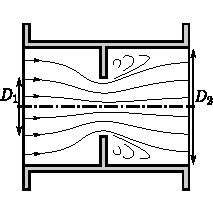
\includegraphics{fig/appendix/Orifice}}}
	\end{tabular}
\end{minipage}
\vspace{1cm}

\begin{minipage}{\textwidth}
	\captionof{table}{Verliescoëfficiënt bij verschillende types instroming \\ $h_\mathrm{L} = K \frac{v_2^2}{2g}$}
	\begin{tabular}[t]{c c c}
		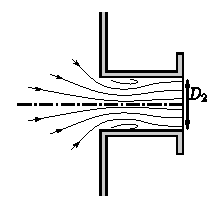
\includegraphics{fig/appendix/Instroming}
		&
		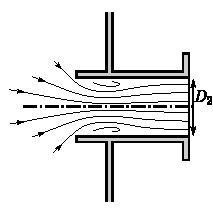
\includegraphics{fig/appendix/Buis_instroming}
		&
		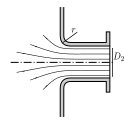
\includegraphics{fig/appendix/Afgeronde_instroming}
		\\
		$K = 0.5$  & $K = 1.0$ & 
		\begin{tabular}{l c c c c c c}
			$r/D_2$ & 0.00 & 0.02 & 0.04 & 0.06 & 0.10 & $>$0.15  \\ 
			\hline
			$K$    & 0.50    & 0.28    & 0.24      & 0.15    & 0.09     & 0.04  \\
		\end{tabular}
	\end{tabular}
\end{minipage}
\vspace{1cm}


%\begin{minipage}{\textwidth}
%	\captionof{table}{Verliescoëfficiënt bij een afgeronde instroming}
%	\begin{tabular}[t]{p{12cm} p{5cm}}
%	
%		$K = 0.50$  & 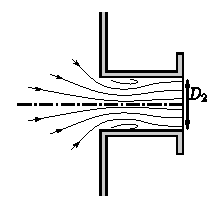
\includegraphics{fig/appendix/Instroming}\\
%		
%		$K = 1.00$  & 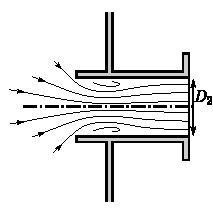
\includegraphics{fig/appendix/Buis_instroming}\\
%		
%		\begin{tabular}{l c c c c c c}
%			$r/D_2$ & 0.00 & 0.02 & 0.04 & 0.06 & 0.10 & $>$0.15  \\ 
%			\hline
%			$K$    & 0.50    & 0.28    & 0.24      & 0.15    & 0.09     & 0.04  \\
%		\end{tabular}
%		&
%		\vfill
%		\smash{\raisebox{-0.5\height}{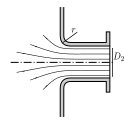
\includegraphics{fig/appendix/Afgeronde_instroming}}}
%	\end{tabular}
%\end{minipage}

\begin{figure}[ht]
	\caption{Moody diagram}
	\label{fig:Moody diagram}
	\centering
	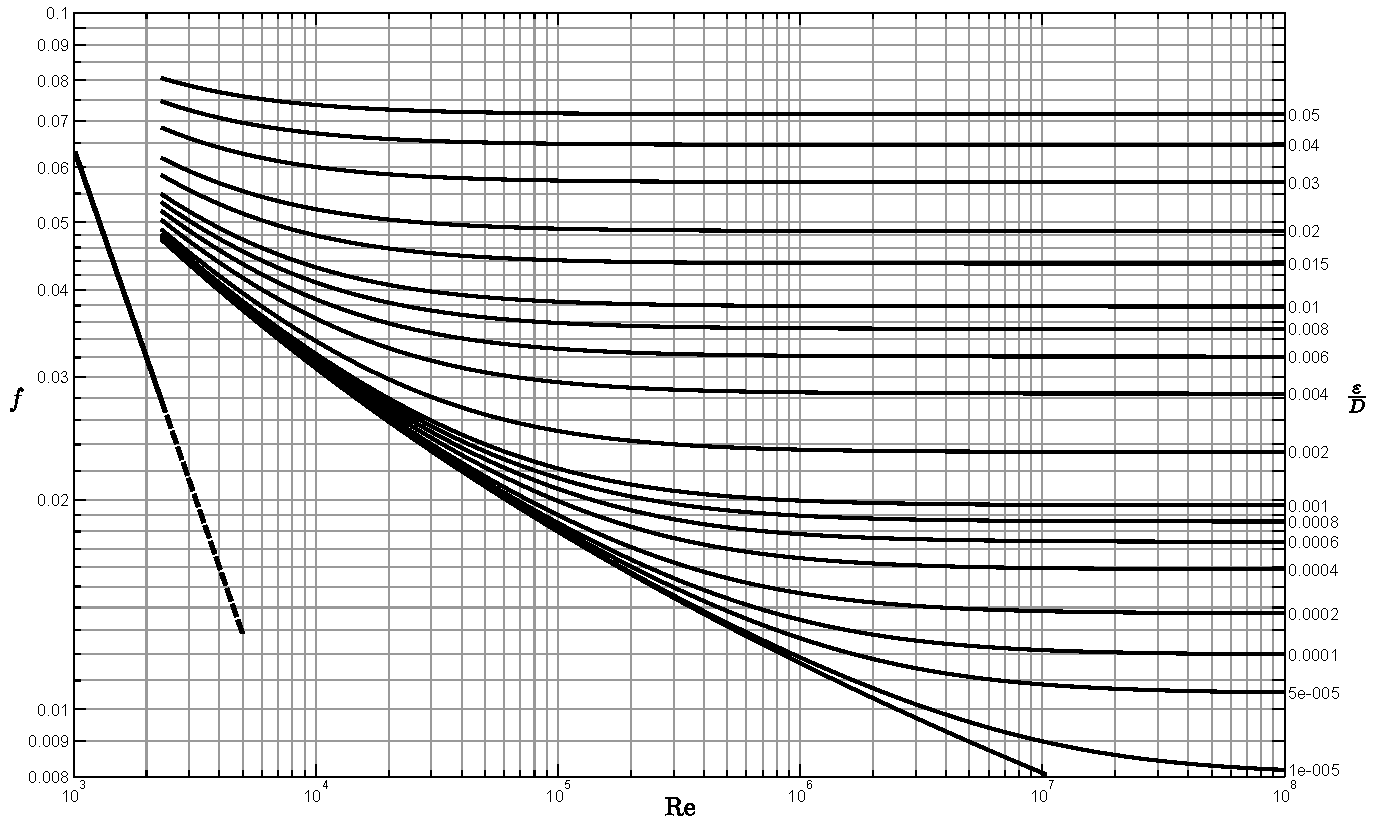
\includegraphics[width=22cm, angle=270]{fig/stroming_in_leidingen/Moody_diagram.pdf}
\end{figure}